\documentclass[../main.tex]{subfiles}




\begin{document}
\chapter{}
\label{cha:cha_18}

\section{}
\begin{enumerate}[label=\bfseries(\alph*)]
\item  The analytical solution can be derived by the separation of variables,
	\bigbreak
$\displaystyle\int \dfrac{d y}{y}=\int t^{3}-1.5 d t$
	\bigbreak
The integrals can be evaluated to give,
	\bigbreak
$\ln y=\dfrac{t^{4}}{4}-1.5 t+C$
	\bigbreak
Substituting the initial conditions yields $C=0$. Substituting this value and taking the exponential gives
	\bigbreak
$y=e^{t^{4} / 4-1.5 t}$
	\bigbreak
\item  Euler method $(h=0.5)$ :
	\bigbreak
\begin{tabular}{crr}
\hline
$\boldsymbol{t}$ & \multicolumn{1}{c}{$\boldsymbol{y}$} & \multicolumn{1}{c}{$d y / d t$} \\
\hline
$\mathbf{0}$ & $\mathbf{1}$ & $-1.5$ \\
$\mathbf{0 . 5}$ & $\mathbf{0 . 2 5}$ & $-0.34375$ \\
$\mathbf{1}$ & $\mathbf{0 . 0 7 8 1 2 5}$ & $-0.03906$ \\
$\mathbf{1 . 5}$ & $\mathbf{0 . 0 5 8 5 9 4}$ & $0.109863$ \\
$\mathbf{2}$ & $\mathbf{0 . 1 1 3 5 2 5}$ &  \\
\hline
\end{tabular}
	\bigbreak
Euler method $(h=0.25):$
	\bigbreak
\begin{tabular}{crr}
\hline
$\boldsymbol{t}$ & \multicolumn{1}{c}{$\boldsymbol{y}$} & \multicolumn{1}{c}{$d y / d t$} \\
\hline
$\mathbf{0}$ & $\mathbf{1}$ & $-1.5$ \\
$\mathbf{0 . 2 5}$ & $\mathbf{0 . 6 2 5}$ & $-0.92773$ \\
$\mathbf{0 . 5}$ & $\mathbf{0 . 3 9 3 0 6 6}$ & $-0.54047$ \\
$\mathbf{0 . 7 5}$ & $\mathbf{0 . 2 5 7 9 5}$ & $-0.2781$ \\
$\mathbf{1}$ & $\mathbf{0 . 1 8 8 4 2 4}$ & $-0.09421$ \\
$\mathbf{1 . 2 5}$ & $\mathbf{0 . 1 6 4 8 7 1}$ & $0.074707$ \\
$\mathbf{1 . 5}$ & $\mathbf{0 . 1 8 3 5 4 8}$ & $0.344153$ \\
$\mathbf{1 . 7 5}$ & $\mathbf{0 . 2 6 9 5 8 6}$ & $1.040434$ \\
$\mathbf{2}$ & $\mathbf{0 . 5 2 9 6 9 5}$ &  \\
\hline
\end{tabular}
	\bigbreak
\item Midpoint method $(h=0.5)$
	\bigbreak
\begin{tabular}{crrrrr}
\hline
$\boldsymbol{t}$ & $\boldsymbol{y}$ & $d y / d t$ & $t_{m}$ & $y_{m}$ & $d y_{m} / d t$ \\
\hline
$\mathbf{0}$ & $\mathbf{1}$ & $-1.5$ & $0.25$ & $0.625$ & $-0.92773$ \\
$\mathbf{0 . 5}$ & $\mathbf{0 . 5 3 6 1 3 3}$ & $-0.73718$ & $0.75$ & $0.351837$ & $-0.37932$ \\
$\mathbf{1}$ & $\mathbf{0 . 3 4 6 4 7 1}$ & $-0.17324$ & $1.25$ & $0.303162$ & $0.13737$ \\
$\mathbf{1 . 5}$ & $\mathbf{0 . 4 1 5 1 5 6}$ & $0.778417$ & $1.75$ & $0.60976$ & $2.353292$ \\
$\mathbf{2}$ & $\mathbf{1 . 5 9 1 8 0 2}$ &  &  &  &  \\
\hline
\end{tabular}
	\bigbreak
\item RK4 $(h=0.5)$
	\bigbreak
\begin{tabular}{ccccccccccccc}
\hline
$\boldsymbol{t}$ & $\boldsymbol{y}$ & $k_{1}$ & $t_{m}$ & $y_{m}$ & $k_{2}$ & $t_{m}$ & $y_{m}$ & $k_{3}$ & $t_{e}$ & $y_{e}$ & $k_{4}$ & $\phi$\\
\hline
$\mathbf{0}$ & $\mathbf{1 . 0 0 0 0}$ & $-1.5000$ & $0.25$ & $0.6250$ & $-0.9277$ & $0.25$ & $0.7681$ & $-1.1401$ & $0.5$ & $0.4300$ & $-0.5912$ & $-1.0378$\\
$\mathbf{0 . 5}$ & $\mathbf{0 . 4 8 1 1}$ & $-0.6615$ & $0.75$ & $0.3157$ & $-0.3404$ & $0.75$ & $0.3960$ & $-0.4269$ & 1 & $0.2676$ & $-0.1338$ & $-0.3883$\\
$\mathbf{1}$ & $\mathbf{0 . 2 8 6 9}$ & $-0.1435$ & $1.25$ & $0.2511$ & $0.1138$ & $1.25$ & $0.3154$ & $0.1429$ & $1.5$ & $0.3584$ & $0.6720$ & $0.1736$\\
$\mathbf{1 . 5}$ & $\mathbf{0 . 3 7 3 8}$ & $0.7008$ & $1.75$ & $0.5489$ & $2.1186$ & $1.75$ & $0.9034$ & $3.4866$ & 2 & $2.1170$ & $13.7607$ & $4.2786$\\
$\mathbf{2}$ & $\mathbf{2 . 5 1 3 1}$ &  &  &  &  &  &  &  &  &  &  & \\
\hline
\end{tabular}
	\bigbreak
All the solutions can be presented graphically as
	\bigbreak
	\begin{figure}[H]
		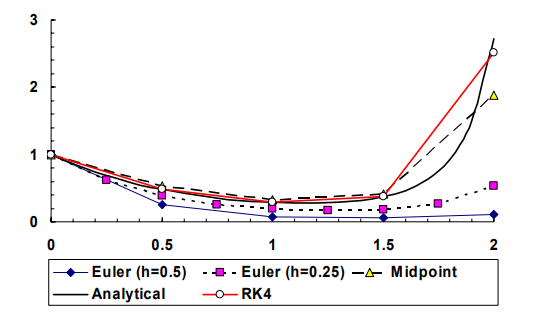
\includegraphics[width=0.5\linewidth]{fig_18_1}
		\label{fig:fig_18_1}
	\end{figure}
\end{enumerate}
	\bigbreak


\section{} \label{sec:sec_18_2}
\begin{enumerate}[label=\bfseries(\alph*)]
\item The analytical solution can be derived by the separation of variables,
	\bigbreak
$\displaystyle\int \dfrac{d y}{\sqrt{y}}=\int 1+2 x d x$
	\bigbreak
The integrals can be evaluated to give,
	\bigbreak
$2 \sqrt{y}=x+x^{2}+C$
	\bigbreak
Substituting the initial conditions yields $C=2$. Substituting this value and rearranging gives
	\bigbreak
$y=\left(\dfrac{x^{2}+x+2}{2}\right)^{2}$
	\bigbreak
Some selected value can be computed as
	\bigbreak
\begin{tabular}{rr}
\hline
\multicolumn{1}{c}{$x$} & $y$ \\
\hline
0 & 1 \\
$0.25$ & $1.336914$ \\
$0.5$ & $1.890625$ \\
$0.75$ & $2.743164$ \\
$1 $ & $4$\\
\hline
\end{tabular}
	\bigbreak
\item Euler's method:
	\bigbreak
$y(0.25)=y(0)+f(0,1) h$
	\bigbreak
$f(0,1)=(1+2(0)) \sqrt{1}=1$
	\bigbreak
$y(0.25)=1+1(0.25)=1.25$
	\bigbreak
$y(0.5)=y(0.25)+f(0.25,1.25) 0.25$
	\bigbreak
$f(0.25,1.25)=(1+2(0.25)) \sqrt{1.25}=1.67705$
	\bigbreak
$y(0.5)=1.25+1.67705(0.25)=1.66926$
	\bigbreak
The remaining steps can be implemented and summarized as
	\bigbreak
\begin{tabular}{crr}
\hline
$\boldsymbol{x}$ & \multicolumn{1}{c}{$\boldsymbol{y}$} & \multicolumn{1}{c}{$d y / d x$} \\
\hline
$\mathbf{0}$ & $\mathbf{1}$ & 1 \\
$\mathbf{0 . 2 5}$ & $\mathbf{1 . 2 5}$ & $1.67705$ \\
$\mathbf{0 . 5}$ & $\mathbf{1 . 6 6 9 2 6}$ & $2.584$ \\
$\mathbf{0 . 7 5}$ & $\mathbf{2 . 3 1 5 2 6}$ & $3.804$ \\
$\mathbf{1}$ & $\mathbf{3 . 2 6 6 2 6}$ & $5.42184$ \\
\hline
\end{tabular}
	\bigbreak
\item Heun's method:
	\bigbreak
Predictor:
	\bigbreak
$k_{1}=(1+2(0)) \sqrt{1}=1$
	\bigbreak
$y(0.25)=1+1(0.25)=1.25$
	\bigbreak
$k_{2}=(1+2(0.25)) \sqrt{1.25}=1.6771$
	\bigbreak
Corrector:
	\bigbreak
$y(0.25)=1+\dfrac{1+1.6771}{2} 0.25=1.33463$
	\bigbreak
The remaining steps can be implemented and summarized as
	\bigbreak
\begin{tabular}{rrcrrrr}
\hline
\multicolumn{1}{c}{$\boldsymbol{x}$} & $\boldsymbol{y}$ & $k_{1}$ & \multicolumn{1}{c}{$x_{e}$} & \multicolumn{1}{c}{$y_{e}$} & $k_{2}$ & $d y / d x$ \\
\hline
$\mathbf{0}$ & $\mathbf{1}$ & $1.0000$ & $0.25$ & $1.25$ & $1.6771$ & $1.3385$ \\
$\mathbf{0 . 2 5}$ & $\mathbf{1 . 3 3 4 6 3}$ & $1.7329$ & $0.5$ & $1.76785$ & $2.6592$ & $2.1961$ \\
$\mathbf{0 . 5}$ & $\mathbf{1 . 8 8 3 6 4}$ & $2.7449$ & $0.75$ & $2.56987$ & $4.0077$ & $3.3763$ \\
$\mathbf{0 . 7 5}$ & $\mathbf{2 . 7 2 7 7 2}$ & $4.1290$ & 1 & $3.75996$ & $5.8172$ & $4.9731$ \\
$\mathbf{1}$ & $\mathbf{3 . 9 7 0 9 9}$ &  &  &  &  &  \\
\hline
\end{tabular}
	\bigbreak
\item Ralston's method:
	\bigbreak
Predictor:
	\bigbreak
$k_{1}=(1+2(0)) \sqrt{1}=1$
	\bigbreak
$y(0.1875)=1+1(0.1875)=1.1875$
	\bigbreak
$k_{2}=(1+2(0.1875)) \sqrt{1.1875}=1.49837$
	\bigbreak
Corrector:
	\bigbreak
$y(0.25)=1+\dfrac{1+2(1.49837)}{3} 0.25=1.33306$
	\bigbreak
The remaining steps can be implemented and summarized as
	\bigbreak
\begin{tabular}{rrrrrrr}
\hline
\multicolumn{1}{r}{$\boldsymbol{x}$} & $\boldsymbol{y}$ & \multicolumn{1}{c}{$k_{1}$} & $x+3 / 4 h$ & $y+(3 / 4) k_{1} h$ & $k_{2}$ & $d y / d x$ \\
\hline
$\mathbf{0}$ & $\mathbf{1}$ & 1 & $0.1875$ & $1.1875$ & $1.49837$ & $1.3322$ \\
$\mathbf{0 . 2 5}$ & $\mathbf{1 . 3 3 3 0 6}$ & $1.73187$ & $0.4375$ & $1.65779$ & $2.41416$ & $2.1867$ \\
$\mathbf{0 . 5}$ & $\mathbf{1 . 8 7 9 7 4}$ & $2.74208$ & $0.6875$ & $2.39388$ & $3.67464$ & $3.3638$ \\
$\mathbf{0 . 7 5}$ & $\mathbf{2 . 7 2 0 6 9}$ & $4.12363$ & $0.9375$ & $3.49387$ & $5.37392$ & $4.9572$ \\
$\mathbf{1}$ & $\mathbf{3 . 9 5 9 9 8}$ &  &  &  &  &  \\
\hline
\end{tabular}
	\bigbreak
\item RK4
	\bigbreak
\begin{tabular}{ccccccccccccc}
\hline
$\boldsymbol{x}$ & $\boldsymbol{y}$ & $k_{1}$ & $x_{m}$ & $y_{m}$ & $k_{2}$ & $x_{m}$ & $y_{m}$ & $k_{3}$ & $x_{e}$ & $y_{e}$ & $k_{4}$ & $\phi$\\
\hline
$\mathbf{0}$&$\mathbf{1.0000}$&1&0.125&1.1250&1.32583&0.125&1.1657&1.34961&0.25&1.3374&1.73469&1.3476\\
$\mathbf{0.25}$&$\mathbf{1.3369}$&1.73436&0.375&1.5537&2.18133&0.375&1.6096&2.2202&0.5&1.8919&2.75096&2.2147\\
$\mathbf{0.5}$&$\mathbf{1.8906}$&2.74997&0.625&2.2343&3.36322&0.625&2.3110&3.42043&0.75&2.7457&4.14253&3.4100\\
$\mathbf{0.75}$&$\mathbf{2.7431}$&4.14056&0.875&3.2606&4.96574&0.875&3.3638&5.04368&1&4.0040&6.00299&5.0271\\
 $\mathbf{1}$  $\mathbf{3.9998}$ &  &  &  &  &  &  &  &  &  &  & \\
\hline
\end{tabular}
	\bigbreak
	\begin{figure}[H]
		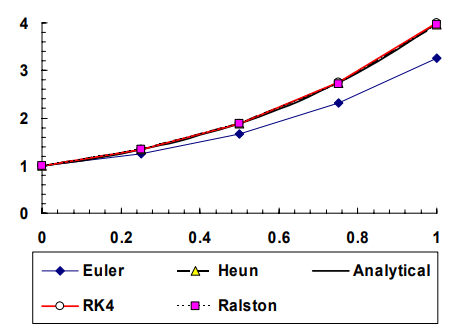
\includegraphics[width=0.5\linewidth]{fig_18_2}
		\label{fig:fig_18_2}
	\end{figure}
\end{enumerate}



\section{}
\begin{enumerate}[label=\bfseries(\alph*)]
\item\label{enu:enu18_2_1} Heun's method:
	\bigbreak
Predictor:
	\bigbreak
$k_{1}=-2(1)+(0)^{2}=-2$
	\bigbreak
$y(0.5)=1+(-2)(0.5)=0$
	\bigbreak
$k_{2}=-2(0)+0.5^{2}=0.25$
	\bigbreak
The remaining steps can be implemented and summarized as
	\bigbreak
\begin{tabular}{|r|r|r|r|r|r|r|}
\hline
\multicolumn{1}{|c|}{$\boldsymbol{t}$} & \multicolumn{1}{c|}{$\boldsymbol{y}$} & $k_{1}$ & $x_{i+1}$ & \multicolumn{1}{c|}{$y_{i+1}$} & \multicolumn{1}{|c|}{$k_{2}$} & \multicolumn{1}{c|}{$d y / d t$} \\
\hline
$\mathbf{0}$ & $\mathbf{1}$ & $-2.0000$ & $0.5$ & 0 & $0.2500$ & $-0.875$ \\
\hline
$\mathbf{0 . 5}$ & $\mathbf{0 . 5 6 2 5}$ & $-0.8750$ & 1 & $0.125$ & $0.7500$ & $-0.0625$ \\
\hline
$\mathbf{1}$ & $\mathbf{0 . 5 3 1 2 5}$ & $-0.0625$ & $1.5$ & $0.5$ & $1.2500$ & $0.59375$ \\
\hline
$\mathbf{1 . 5}$ & $\mathbf{0 . 8 2 8 1 3}$ & $0.5938$ & 2 & $1.125$ & $1.7500$ & $1.17188$ \\
\hline
$\mathbf{2}$ & $\mathbf{1 . 4 1 4 0 6}$ & $1.1719$ &  &  &  &  \\
\hline
\end{tabular}
	\bigbreak
\item As in Part \ref{enu:enu18_2_1}, the corrector can be represented as
	\bigbreak
$y_{i+1}^{1}=1+\dfrac{-2+\left(-2(0)+0.5^{2}\right)}{2} 0.5=0.5625$
	\bigbreak
The corrector can then be iterated to give
	\bigbreak
$y_{i+1}^{2}=1+\dfrac{-2+\left(-2(0.5625)+0.5^{2}\right)}{2} 0.5=0.28125$
	\bigbreak
$y_{i+1}^{3}=1+\dfrac{-2+\left(-2(0.28125)+0.5^{2}\right)}{2} 0.5=0.421875$
	\bigbreak
The iterations can be continued until the percent relative error falls below $0.1 \%$. This occurs after 12 iterations with the result that $y(0.5)=0.37491$ with $\varepsilon_{a}=0.073 \%$. The remaining values can be computed in a like fashion to give
	\bigbreak
\begin{tabular}{cc}
\hline
$\boldsymbol{t}$&$\boldsymbol{y}$\\
\hline
$\mathbf{0}$&$\mathbf{1.0000000}$\\
$\mathbf{0.5}$&$\mathbf{0.3749084}$\\
$\mathbf{1}$&$\mathbf{0.3334045}$\\
$\mathbf{1.5}$&$\mathbf{0.6526523}$\\
$\mathbf{2}$&$\mathbf{1.2594796}$\\
\hline
\end{tabular}
	\bigbreak
\item  Midpoint method
	\bigbreak
$k_{1}=-2(1)+(0)^{2}=-2$
	\bigbreak
$y(0.25)=1+(-2)(0.25)=0.5$
	\bigbreak
$k_{2}=-2(0.5)+0.25^{2}=-0.9375$
	\bigbreak
$y(0.5)=1+(-0.9375) 0.5=0.53125$
	\bigbreak
The remainder of the computations can be implemented in a similar fashion as listed below:
	\bigbreak
\begin{tabular}{rrlrrr}
\hline
\multicolumn{1}{c}{$\boldsymbol{t}$} & $\boldsymbol{y}$ & \multicolumn{1}{c}{$d y / d t$} & $t_{m}$ & \multicolumn{1}{c}{$y_{m}$} & $d y_{m} / d t$ \\
\hline
$\mathbf{0}$ & $\mathbf{1}$ & $-2.0000$ & $0.25$ & $0.5$ & $-0.9375$ \\
$\mathbf{0 . 5}$ & $\mathbf{0 . 5 3 1 2 5}$ & $-0.8125$ & $0.75$ & $0.328125$ & $-0.0938$ \\
$\mathbf{1}$ & $\mathbf{0 . 4 8 4 3 8}$ & $0.0313$ & $1.25$ & $0.492188$ & $0.57813$ \\
$\mathbf{1 . 5}$ & $\mathbf{0 . 7 7 3 4 4}$ & $0.7031$ & $1.75$ & $0.949219$ & $1.16406$ \\
$\mathbf{2}$ & $\mathbf{1 . 3 5 5 4 7}$ &  &  &  &  \\
\hline
\end{tabular}
	\bigbreak
\item Ralston's method:
	\bigbreak
$k_{1}=-2(1)+(0)^{2}=-2$
	\bigbreak
$y(0.375)=1+(-2)(0.375)=0.25$
	\bigbreak
$k_{2}=-2(0.25)+0.375^{2}=-0.3594$
	\bigbreak
$y(0.25)=1+\dfrac{-2+2(-0.3594)}{3} 0.5=0.54688$
	\bigbreak
The remaining steps can be implemented and summarized as
	\bigbreak
\begin{tabular}{rrrrrrr}
\hline
\multicolumn{1}{c}{$\boldsymbol{t}$} & $\boldsymbol{y}$ & $k_{1}$ & $t+3 / 4 h$ & $y+(3 / 4) k_{1} h$ & $k_{2}$ & $d y / d t$ \\
\hline
$\mathbf{0}$ & $\mathbf{1}$ & $-2.0000$ & $0.375$ & $0.25$ & $-0.3594$ & $-0.9063$ \\
$\mathbf{0 . 5}$ & $\mathbf{0 . 5 4 6 8 8}$ & $-0.8438$ & $0.875$ & $0.230469$ & $0.3047$ & $-0.0781$ \\
$\mathbf{1}$ & $\mathbf{0 . 5 0 7 8 1}$ & $-0.0156$ & $1.375$ & $0.501953$ & $0.8867$ & $0.58594$ \\
$\mathbf{1 . 5}$ & $\mathbf{0 . 8 0 0 7 8}$ & $0.6484$ & $1.875$ & $1.043945$ & $1.4277$ & $1.16797$ \\
$\mathbf{2}$ & $\mathbf{1 . 3 8 4 7 7}$ &  &  &  &  &  \\
\hline
\end{tabular}
\end{enumerate}
	\bigbreak
All the versions can be plotted as:
	\bigbreak
	\begin{figure}[H]
		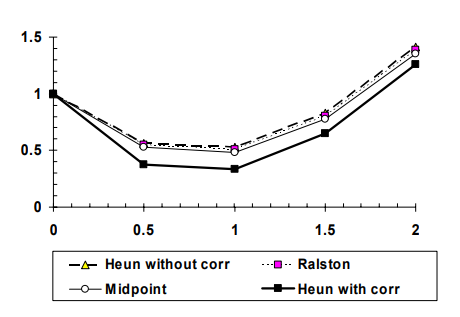
\includegraphics[width=0.5\linewidth]{fig_18_3}
		\label{fig:fig_18_3}
	\end{figure}
	\bigbreak



\section{}
\begin{enumerate}[label=\bfseries(\alph*)]
\item The solution to the differential equation is
	\bigbreak
$p=p_{0} e^{k_{g} t}$
	\bigbreak
Taking the natural log of this equation gives
	\bigbreak
$\ln p=\ln p_{0}+k_{g} t$
	\bigbreak
Therefore, a semi-log plot ( $\ln p$ versus $t$ ) should yield a straight line with a slope of $k_{g}$. The plot, along with the linear regression best fit line is shown below. The estimate of the population growth rate is $k_{g}=0.0178 / y r$.
	\bigbreak
	\begin{figure}[H]
		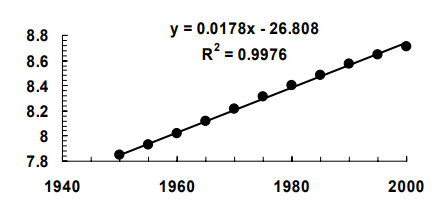
\includegraphics[width=0.5\linewidth]{fig_18_4}
		\label{fig:fig_18_4}
	\end{figure}
	\bigbreak
\item The ODE can be integrated with the fourth-order RK method with the results tabulated and plotted below:
	\bigbreak
\begin{tabular}{ccccccccccc}
\hline
$t$ & $p$ & $k_{1}$ & $p_{\text {mid }}$ & $k_{2}$ & $p_{\text {mid }}$ & $k_{3}$ & $p_{\text {end }}$ & $k_{4}$ & $\phi$ \\
\hline
1950 & $2555.00$ & $45.41$ & $2668.53$ & $47.43$ & $2673.58$ & $47.52$ & $2792.60$ & $49.64$ & $47.49$ \\
1955 & $2792.46$ & $49.63$ & $2916.55$ & $51.84$ & $2922.06$ & $51.94$ & $3052.15$ & $54.25$ & $51.91$ \\
1960 & $3051.99$ & $54.25$ & $3187.61$ & $56.66$ & $3193.64$ & $56.76$ & $3335.81$ & $59.29$ & $56.73$ \\
1965 & $3335.64$ & $59.29$ & $3483.87$ & $61.92$ & $3490.45$ & $62.04$ & $3645.84$ & $64.80$ & $62.00$ \\
1970 & $3645.66$ & $64.80$ & $3807.66$ & $67.68$ & $3814.85$ & $67.81$ & $3984.69$ & $70.82$ & $67.77$ \\
1975 & $3984.48$ & $70.82$ & $4161.54$ & $73.97$ & $4169.41$ & $74.11$ & $4355.02$ & $77.41$ & $74.06$ \\
1980 & $4354.80$ & $77.40$ & $4548.31$ & $80.84$ & $4556.91$ & $81.00$ & $4759.78$ & $84.60$ & $80.95$ \\
1985 & $4759.54$ & $84.60$ & $4971.03$ & $88.36$ & $4980.43$ & $88.52$ & $5202.15$ & $92.46$ & $88.47$ \\
1990 & $5201.89$ & $92.46$ & $5433.04$ & $96.57$ & $5443.31$ & $96.75$ & $5685.64$ & $101.06$ & $96.69$ \\
1995 & $5685.35$ & $101.05$ & $5937.98$ & $105.54$ & $5949.21$ & $105.74$ & $6214.06$ & $110.45$ & $105.68$ \\
2000 & $6213.75$ & $110.44$ & $6489.86$ & $115.35$ & $6502.13$ & $115.57$ & $6791.60$ & $120.72$ & $115.50$ \\
2005 & $6791.25$ & $120.71$ & $7093.02$ & $126.07$ & $7106.43$ & $126.31$ & $7422.81$ & $131.93$ & $126.24$ \\
2010 & $7422.43$ & $131.93$ & $7752.25$ & $137.79$ & $7766.90$ & $138.05$ & $8112.68$ & $144.20$ & $137.97$ \\
2015 & $8112.27$ & $144.19$ & $8472.74$ & $150.60$ & $8488.76$ & $150.88$ & $8866.67$ & $157.60$ & $150.79$ \\
2020 & $8866.22$ & $157.59$ & $9260.20$ & $164.59$ & $9277.70$ & $164.90$ & $9690.74$ & $172.25$ & $164.80$ \\
2025 & $9690.24$ & $172.24$ & $10120.84$ & $179.89$ & $10139.97$ & $180.23$ & $10591.40$ & $188.25$ & $180.12$ \\
2030 & $10590.85$ & $188.24$ & $11061.47$ & $196.61$ & $11082.38$ & $196.98$ & $11575.76$ & $205.75$ & $196.86$ \\
2035 & $11575.17$ & $205.74$ & $12089.52$ & $214.88$ & $12112.37$ & $215.29$ & $12651.61$ & $224.87$ & $215.16$ \\
2040 & $12650.96$ & $224.86$ & $13213.11$ & $234.85$ & $13238.09$ & $235.30$ & $13827.45$ & $245.77$ & $235.16$ \\
2045 & $13826.74$ & $245.76$ & $14441.14$ & $256.68$ & $14468.44$ & $257.17$ & $15112.57$ & $268.61$ & $257.01$ \\
2050 & $15111.79$ &  &  &  &  &  &  &  &  \\
\hline
\end{tabular}
	\bigbreak
	\begin{figure}[H]
		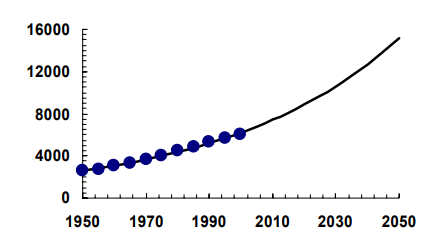
\includegraphics[width=0.5\linewidth]{fig_18_5}
		\label{fig:fig_18_5}
	\end{figure}
	\bigbreak
\end{enumerate}



\section{} \label{sec:sec_18_5}
\begin{enumerate}[label=\bfseries(\alph*)]
\item  The analytical solution can be used to compute values at times over the range. For example, the value at $t=1955$ can be computed as
	\bigbreak
$p=2,555 \dfrac{12,000}{2,555+(12,000-2,555) e^{-0.026(1955-1950)}}=2,826.2$
	\bigbreak
Values at the other times can be computed and displayed along with the data in the plot below.
	\bigbreak
\item The ODE can be integrated with the fourth-order RK method with the results tabulated and plotted below:
	\bigbreak
\begin{tabular}{cccccccccccccc}
\hline
$t$ & $p-r k 4$ & $k_{1}$ & $t_{m}$ & $y_{m}$ & $k_{2}$ & $t_{m}$ & $y_{m}$ & $k_{3}$ & $t_{e}$ & $y_{e}$ & $k_{4}$ & $\phi$ \\
\hline
1950 & $2555.0$ & $52.29$ & $1952.5$ & $2685.7$ & $54.20$ & $1952.5$ & $2690.5$ & $54.27$ & $1955.0$ & $2826.3$ & $56.18$ & $54.23$ \\
1955 & $2826.2$ & $56.17$ & $1957.5$ & $2966.6$ & $58.06$ & $1957.5$ & $2971.3$ & $58.13$ & $1960.0$ & $3116.8$ & $59.99$ & $58.09$ \\
1960 & $3116.6$ & $59.99$ & $1962.5$ & $3266.6$ & $61.81$ & $1962.5$ & $3271.1$ & $61.87$ & $1965.0$ & $3425.9$ & $63.64$ & $61.83$ \\
1965 & $3425.8$ & $63.64$ & $1967.5$ & $3584.9$ & $65.36$ & $1967.5$ & $3589.2$ & $65.41$ & $1970.0$ & $3752.8$ & $67.06$ & $65.37$ \\
1970 & $3752.6$ & $67.06$ & $1972.5$ & $3920.3$ & $68.63$ & $1972.5$ & $3924.2$ & $68.66$ & $1975.0$ & $4096.0$ & $70.15$ & $68.63$ \\
1975 & $4095.8$ & $70.14$ & $1977.5$ & $4271.2$ & $71.52$ & $1977.5$ & $4274.6$ & $71.55$ & $1980.0$ & $4453.5$ & $72.82$ & $71.52$ \\
1980 & $4453.4$ & $72.82$ & $1982.5$ & $4635.4$ & $73.97$ & $1982.5$ & $4638.3$ & $73.98$ & $1985.0$ & $4823.3$ & $75.00$ & $73.95$ \\
1985 & $4823.1$ & $75.00$ & $1987.5$ & $5010.6$ & $75.88$ & $1987.5$ & $5012.8$ & $75.89$ & $1990.0$ & $5202.6$ & $76.62$ & $75.86$ \\
1990 & $5202.4$ & $76.62$ & $1992.5$ & $5394.0$ & $77.20$ & $1992.5$ & $5395.5$ & $77.21$ & $1995.0$ & $5588.5$ & $77.63$ & $77.18$ \\
1995 & $5588.3$ & $77.63$ & $1997.5$ & $5782.4$ & $77.90$ & $1997.5$ & $5783.1$ & $77.90$ & $2000.0$ & $5977.8$ & $78.00$ & $77.87$ \\
2000 & $5977.7$ & $78.00$ & $2002.5$ & $6172.7$ & $77.94$ & $2002.5$ & $6172.5$ & $77.94$ & $2005.0$ & $6367.4$ & $77.71$ & $77.91$ \\
2005 & $6367.2$ & $77.71$ & $2007.5$ & $6561.5$ & $77.32$ & $2007.5$ & $6560.5$ & $77.32$ & $2010.0$ & $6753.8$ & $76.77$ & $77.29$ \\
2010 & $6753.7$ & $76.77$ & $2012.5$ & $6945.6$ & $76.06$ & $2012.5$ & $6943.9$ & $76.07$ & $2015.0$ & $7134.0$ & $75.21$ & $76.04$ \\
2015 & $7133.9$ & $75.21$ & $2017.5$ & $7321.9$ & $74.21$ & $2017.5$ & $7319.4$ & $74.23$ & $2020.0$ & $7505.0$ & $73.09$ & $74.20$ \\
2020 & $7504.9$ & $73.09$ & $2022.5$ & $7687.6$ & $71.83$ & $2022.5$ & $7684.5$ & $71.85$ & $2025.0$ & $7864.2$ & $70.47$ & $71.82$ \\
2025 & $7864.0$ & $70.47$ & $2027.5$ & $8040.2$ & $68.98$ & $2027.5$ & $8036.5$ & $69.01$ & $2030.0$ & $8209.1$ & $67.43$ & $68.98$ \\
2030 & $8208.9$ & $67.43$ & $2032.5$ & $8377.5$ & $65.75$ & $2032.5$ & $8373.3$ & $65.80$ & $2035.0$ & $8537.9$ & $64.04$ & $65.76$ \\
2035 & $8537.7$ & $64.05$ & $2037.5$ & $8697.8$ & $62.23$ & $2037.5$ & $8693.3$ & $62.28$ & $2040.0$ & $8849.1$ & $60.41$ & $62.25$ \\
2040 & $8849.0$ & $60.41$ & $2042.5$ & $9000.0$ & $58.50$ & $2042.5$ & $8995.2$ & $58.56$ & $2045.0$ & $9141.8$ & $56.61$ & $58.53$ \\
2045 & $9141.6$ & $56.62$ & $2047.5$ & $9283.1$ & $54.65$ & $2047.5$ & $9278.2$ & $54.72$ & $2050.0$ & $9415.2$ & $52.73$ & $54.68$ \\
2050 & $9415.0$ &  &  &  &  &  &  &  &  &  &  &  \\
\hline

\end{tabular}
\end{enumerate}
	\bigbreak
	\begin{figure}[H]
		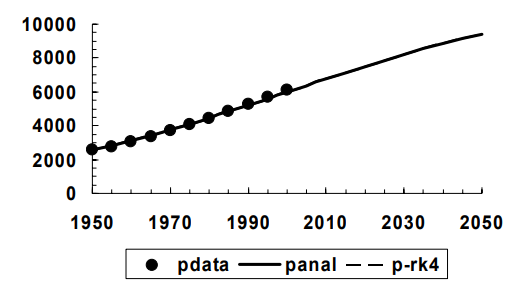
\includegraphics[width=0.5\linewidth]{fig_18_6}
		\label{fig:fig_18_6}
	\end{figure}
	\bigbreak
Thus, the RK4 results are so close to the analytical solution that the two results are indistinguishable graphically.
	\bigbreak



\section{}
\begin{blockquote}
We can solve this problem with the M-file Eulode (Fig.\ref{fig:fig_18_3}). First, we develop a function to compute the derivative
\end{blockquote}
	\bigbreak
\begin{lstlisting}[numbers=none]
function dv = dvdt(t, v)
if t < 10
	% chute is unopened
	dv = 9.81 - 0.25/80*v^2;
else
	% chute is opened
	dv = 9.81 - 5/80*v^2;
end 

\end{lstlisting}
	\bigbreak
\begin{blockquote}
Notice how we have used an If statement to use a higher drag coefficient for times after the cord is pulled. The Eulode function can then be used to generate results and display them graphically..
\end{blockquote}
	\bigbreak
	\begin{figure}[H]
		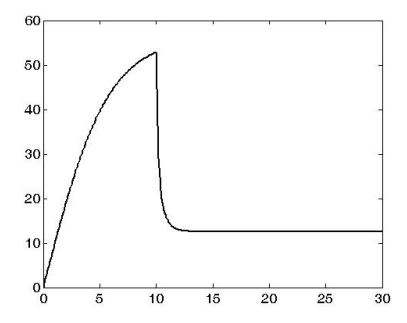
\includegraphics[width=0.5\linewidth]{fig_18_7}
		\label{fig:fig_18_7}
	\end{figure}
	\bigbreak



\section{} \label{sec:sec_18_7}
\begin{enumerate}[label=\bfseries(\alph*)]
\item  Euler's method:
	\bigbreak
\begin{tabular}{rrrrrr}
\multicolumn{1}{c}{$t$} & $y$ & \multicolumn{1}{c}{$z$} & \multicolumn{1}{c}{$d y / d t$} & \multicolumn{1}{c}{$d z / d t$} \\
0 & 2 & 4 & 16 & $-16$ \\
$0.1$ & $3.6$ & $2.4$ & $3.658049$ & $-10.368$ \\
$0.2$ & $3.965805$ & $1.3632$ & $-2.35114$ & $-3.68486$ \\
$0.3$ & $3.730691$ & $0.994714$ & $-3.77687$ & $-1.84568$ \\
$0.4$ & $3.353004$ & $0.810147$ & $-3.99072$ & $-1.10035$ \\
\end{tabular}
	\bigbreak
	\begin{figure}[H]
		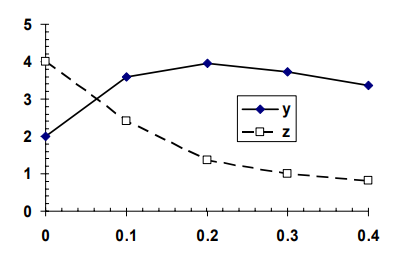
\includegraphics[width=0.5\linewidth]{fig_18_8}
		\label{fig:fig_18_8}
	\end{figure}
	\bigbreak
\item $4^{\text {th }}$-order RK method:
	\bigbreak
$k_{1,1}=f_{1}(0,2,4)=-2(2)+5(4) e^{-0}=16$
	\bigbreak
$k_{1,2}=f_{2}(0,2,4)=-\dfrac{2(4)^{2}}{2}=-16$
	\bigbreak
$y(0.05)=2+16(0.05)=2.8$
	\bigbreak
$z(0.05)=4-16(0.05)=3.2$
	\bigbreak
$k_{2,1}=f_{1}(0.05,2.8,3.2)=-2(2.8)+5(3.2) e^{-0.05}=9.619671 $\bigbreak
$k_{2,2}=f_{2}(0.05,2.8,3.2)=-\dfrac{2.8(3.2)^{2}}{2}=-14.336 $\bigbreak
$y(0.05)=2+9.619671(0.05)=2.480984 $\bigbreak
$z(0.05)=4-14.336(0.05)=3.2832 $\bigbreak
$k_{3,1}=f_{1}(0.05,2.480984,3.2832)=-2(2.480984)+5(3.2832) e^{-0.05}=10.65342 $\bigbreak
$k_{3,2}=f_{2}(0.05,2.480984,3.2832)=-\dfrac{2.480984(3.2832)^{2}}{2}=-13.3718 $\bigbreak
$y(0.1)=2+10.65342(0.1)=3.065342 $\bigbreak
$z(0.1)=4-13.3718(0.1)=2.662824 $\bigbreak
$k_{4,1}=f_{1}(0.1,3.065342,2.662824)=-2(3.065342)+5(3.2832) e^{-0.1}=5.916431 $\bigbreak
$k_{4,2}=f_{2}(0.1,3.065342,2.662824)=-\dfrac{3.065342(2.662824)^{2}}{2}=-10.8676$\bigbreak
	\bigbreak
The $k$ 's can then be used to compute the increment functions,
	\bigbreak
$\phi_{1}=\dfrac{16+2(9.619671+10.65342)+5.916431}{6}=10.41043$
	\bigbreak
$\phi_{2}=\dfrac{-16+2(-14.336-13.3718)-10.8676}{6}=-13.7139$
	\bigbreak
These slope estimates can then be used to make the prediction for the first step
	\bigbreak
$y(0.1)=2+10.41043(0.1)=3.041043$
	\bigbreak
$z(0.1)=4-13.7139(0.1)=2.628615$
	\bigbreak
The remaining steps can be taken in a similar fashion and the results summarized as
	\bigbreak
\begin{tabular}{crr}
\hline
$t$ & $y$ & $z$ \\
\hline
0 & 2 & 4 \\
$0.1$ & $3.041043$ & $2.628615$ \\
$0.2$ & $3.342571$ & $1.845308$ \\
$0.3$ & $3.301983$ & $1.410581$ \\
$0.4$ & $3.107758$ & $1.149986$ \\
\hline
\end{tabular}
	\bigbreak
A plot of these values can be developed.
	\bigbreak
	\begin{figure}[H]
		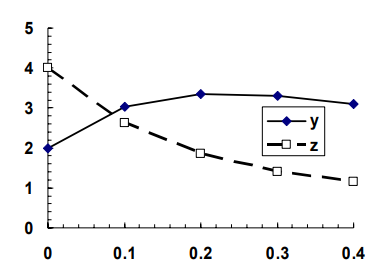
\includegraphics[width=0.5\linewidth]{fig_18_9}
		\label{fig:fig_18_9}
	\end{figure}
\end{enumerate}
	\bigbreak



\section{}
The second-order van der Pol equation can be reexpressed as a system of 2 first-order ODEs,
	\bigbreak
$\dfrac{d y}{d t}=z$
	\bigbreak
$\dfrac{d z}{d t}=\left(1-y^{2}\right) z-y$
	\bigbreak
\begin{enumerate}[label=\bfseries(\alph*)]
\item Euler $(h=0.2)$. Here are the first few steps. The remainder of the computation would be implemented in a similar fashion and the results displayed in the plot below.
	\bigbreak
\begin{tabular}{crrrr}
\hline
$t$ & $y(h=0.2)$ & $z(h=0.2)$ & \multicolumn{1}{c}{$d y / d t$} & \multicolumn{1}{c}{$d z / d t$} \\
\hline
0 & 1 & 1 & 1 & $-1$ \\
$0.2$ & $1.2$ & $0.8$ & $0.8$ & $-1.552$ \\
$0.4$ & $1.36$ & $0.4896$ & $0.4896$ & $-1.77596$ \\
$0.6$ & $1.45792$ & $0.1344072$ & $0.134407$ & $-1.6092$ \\
$0.8$ & $1.4848014$ & $-0.187433$ & $-0.18743$ & $-1.25901$ \\
\hline
\end{tabular}
	\bigbreak
\item Euler $(h=0.1)$. Here are the first few steps. The remainder of the computation would be implemented in a similar fashion and the results displayed in the plot below.
	\bigbreak
\begin{tabular}{rrrrr}
\hline
$t$ & $y(h=0.1)$ & $z(h=0.1)$ & $d y / d t$ & \multicolumn{1}{c}{$d z / d t$} \\
\hline
0 & 1 & 1 & 1 & $-1$ \\
$0.1$ & $1.1$ & $0.9$ & $0.9$ & $-1.289$ \\
$0.2$ & $1.19$ & $0.7711$ & $0.7711$ & $-1.51085$ \\
$0.3$ & $1.26711$ & $0.6200145$ & $0.620015$ & $-1.64257$ \\
$0.4$ & $1.3291115$ & $0.4557574$ & $0.455757$ & $-1.67847$ \\
\hline
\end{tabular}
	\bigbreak
	\begin{figure}[H]
		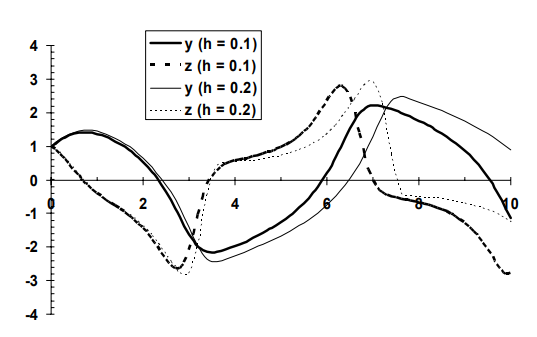
\includegraphics[width=0.5\linewidth]{fig_18_10}
		\label{fig:fig_18_10}
	\end{figure}
	\bigbreak
\end{enumerate}



\section{}
The second-order equation can be reexpressed as a system of two first-order ODEs,
	\bigbreak
$\dfrac{d y}{d t}=z$
	\bigbreak
$\dfrac{d z}{d t}=-9 y$
	\bigbreak
\begin{enumerate}[label=\bfseries(\alph*)]
\item Euler. Here are the first few steps along with the analytical solution. The remainder of the computation would be implemented in a similar fashion and the results displayed in the plot below.
	\bigbreak
\begin{tabular}{rrrrrr}
\hline
\multicolumn{1}{c}{$t$} & \multicolumn{1}{c}{$y_{\text {Euler }}$} & \multicolumn{1}{l}{$Z_{\text {Euler }}$} & \multicolumn{1}{l}{$d y / d t$} & \multicolumn{1}{l}{$d z / d t$} & \multicolumn{1}{l}{$y_{\text {analytical }}$} \\
\hline
0 & 1 & 0 & 0 & $-9$ & 1 \\
$0.1$ & 1 & $-0.9$ & $-0.9$ & $-9$ & $0.955336$ \\
$0.2$ & $0.91$ & $-1.8$ & $-1.8$ & $-8.19$ & $0.825336$ \\
$0.3$ & $0.73$ & $-2.619$ & $-2.619$ & $-6.57$ & $0.62161$ \\
$0.4$ & $0.4681$ & $-3.276$ & $-3.276$ & $-4.2129$ & $0.362358$ \\
\hline
\end{tabular}
	\bigbreak
	\begin{figure}[H]
		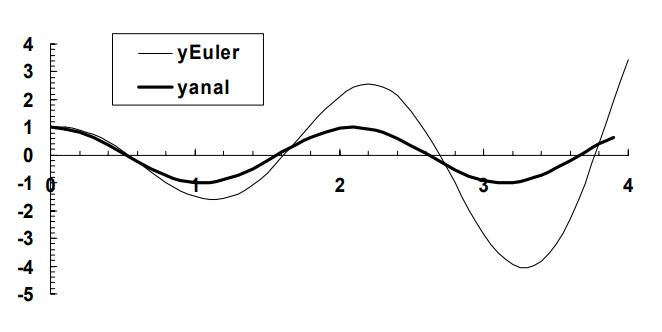
\includegraphics[width=0.5\linewidth]{fig_18_11}
		\label{fig:fig_18_11}
	\end{figure}
	\bigbreak
\item RK4. Here are the first few steps along with the analytical solution. The remainder of the computation would be implemented in a similar fashion and the results displayed in the plot below.
	\bigbreak
$k_{1,1}=f_{1}(0,1,0)=z=0 $\bigbreak
$k_{1,2}=f_{2}(0,1,0)=-9 y=-9(1)=-9 $\bigbreak
$y(0.05)=1+0(0.05)=1 $\bigbreak
$z(0.05)=0-9(0.05)=-0.45 $\bigbreak
$k_{2,1}=f_{1}(0.05,1,-0.45)=-0.45 $\bigbreak
$k_{2,2}=f_{2}(0.05,1,-0.45)=-9(1)=-9 $\bigbreak
$y(0.05)=1+(-0.45)(0.05)=0.9775 $\bigbreak
$z(0.05)=0-9(0.05)=-0.45 $\bigbreak
$k_{3,1}=f_{1}(0.05,0.9775,-0.45)=-0.45 $\bigbreak
$k_{3,2}=f_{2}(0.05,0.9775,-0.45)=-9(0.9775)=-8.7975 $\bigbreak
$y(0.1)=1+(-0.45)(0.1)=0.9550 $\bigbreak
$z(0.1)=0-8.7975(0.1)=-0.8798 $\bigbreak
$k_{4,1}=f_{1}(0.1,0.9550,-0.8798)=-0.8798 $\bigbreak
$k_{4,2}=f_{2}(0.1,0.9550,-0.8798)=-9(0.9550)=-8.5950$\bigbreak
	\bigbreak
The $k$ 's can then be used to compute the increment functions,
	\bigbreak
$\phi_{1}=\dfrac{0+2(-0.45-0.45)-0.8798}{6}=-0.4466$
	\bigbreak
$\phi_{2}=\dfrac{-9+2(-9-8.7975)-8.5950}{6}=-8.8650$
	\bigbreak
These slope estimates can then be used to make the prediction for the first step
	\bigbreak
y(0.1)=1-0.4466(0.1)=0.9553
	\bigbreak
z(0.1)=0-8.8650(0.1)=-0.8865
	\bigbreak
The remaining steps can be taken in a similar fashion and the first few results summarized as
	\bigbreak
\begin{tabular}{rlrl}
\hline
\multicolumn{1}{l}{$t$} & $y$ & \multicolumn{1}{c}{$z$} & $y_{\text {anal }}$ \\
\hline
0 & $1.0000$ & $0.0000$ & $1.00000$ \\
$0.1$ & $0.9553$ & $-0.8865$ & $0.95534$ \\
$0.2$ & $0.8253$ & $-1.6938$ & $0.82534$ \\
$0.3$ & $0.6216$ & $-2.3498$ & $0.62161$ \\
$0.4$ & $0.3624$ & $-2.7960$ & $0.36236$ \\
$0.5$ & $0.0708$ & $-2.9924$ & $0.07074$ \\
\hline
\end{tabular}
	\bigbreak
As can be seen, the results agree with the analytical solution closely. A plot of all the values can be developed and indicates the same close agreement.
	\bigbreak
	\begin{figure}[H]
		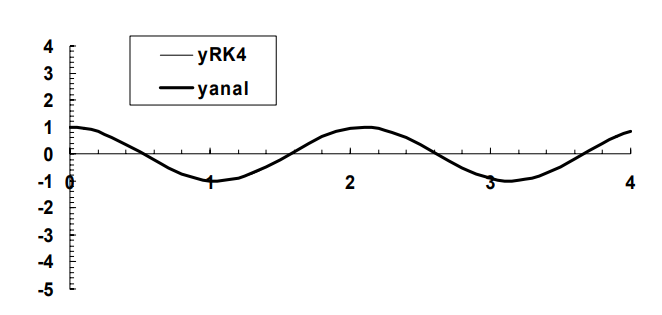
\includegraphics[width=0.5\linewidth]{fig_18_12}
		\label{fig:fig_18_12}
	\end{figure}
	\bigbreak
\end{enumerate}



\section{}
A MATLAB M-file for Heun's method with iteration can be developed as
\begin{lstlisting}[numbers=none]
function [t,y] = Heun(dydt,tspan,y0,h,es,maxit)
% [t,y] = Heun(dydt,tspan,y0,h):
% 	uses the midpoint method to integrate an ODE
% input:
% 	dydt = name of the M-file that evaluates the ODE
% 	tspan = [ti, tf] where ti and tf = initial and
% 		final values of independent variable
% 	y0 = initial value of dependent variable
%	 h = step size
% 	es = stopping criterion (%)
% 		optional (default = 0.001)
%	 maxit = maximum iterations of corrector
% 		optional (default = 50)
% 	es = (optional) stopping criterion (%)
% 	maxit = (optional) maximum allowable iterations
% output:
%	 t = vector of independent variable
%	 y = vector of solution for dependent variable


% if necessary, assign default values
if nargin<6, maxit = 50; end %if maxit blank set to 50
if nargin<5, es = 0.001; end %if es blank set to 0.001
ti = tspan(1);
tf = tspan(2);
t = (ti:h:tf)';
n = length(t);
% if necessary, add an additional value of t
% so that range goes from t = ti to tf
if t(n)<tf
 	t(n+1) = tf;
 	n = n+1;
end
y = y0*ones(n,1); %preallocate y to improve efficiency
iter = 0;
for i = 1:n-1
	 hh = t(i+1) - t(i);
 	k1 = feval(dydt,t(i),y(i));
 	y(i+1) = y(i) + k1*hh;
 	while (1)
 		yold = y(i+1);
 		k2 = feval(dydt,t(i)+hh,y(i+1));
 		y(i+1) = y(i) + (k1+k2)/2*hh;
 		iter = iter + 1;
 		if y(i+1) ~= 0, ea = abs((y(i+1) - yold)/y(i+1)) * 100; end
 		if ea <= es | iter >= maxit, break, end
	 end
end
plot(t,y) 
\end{lstlisting}
	\bigbreak
Here is the test of the solution of Prob.\ref{sec:sec_18_5}. First, an M-file holding the differential
equation is written as
	\bigbreak
\begin{lstlisting}[numbers=none]
function dp = dpdt(t, p)
dp = 0.026*(1-p/12000)*p; 
\end{lstlisting}
	\bigbreak
Then the M-file can be invoked as in
	\bigbreak
\begin{lstlisting}[numbers=none]
>> [t,p]=Heun(@dpdt,[1950 2000],2555,5,0.1);
>> disp([t,p])
 1.0e+003 *

 	 1.9500	 2.5550
	 1.9550	 2.8261
	 1.9600	 3.1165
	 1.9650	 3.4256
	 1.9700	 3.7523
	 1.9750	 4.0953
	 1.9800	 4.4527
	 1.9850	 4.8222
	 1.9900	 5.2012
	 1.9950	 5.5868
	 2.0000	 5.9759 

\end{lstlisting}
	\bigbreak
The following plot is generated
	\bigbreak
	\begin{figure}[H]
		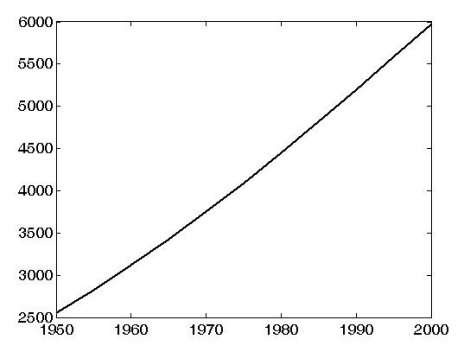
\includegraphics[width=0.5\linewidth]{fig_18_13}
		\label{fig:fig_18_13}
	\end{figure}
	\bigbreak



\section{}
A MATLAB M-file for the midpoint method can be developed as 
	\bigbreak
\begin{lstlisting}[numbers=none]
function [t,y] = midpoint(dydt,tspan,y0,h)
%	 [t,y] = midpoint(dydt,tspan,y0,h):
%	 uses the midpoint method to integrate an ODE
% input:
%	 dydt = name of the M-file that evaluates the ODE
% 	tspan = [ti, tf] where ti and tf = initial and
% 		final values of independent variable
% 	y0 = initial value of dependent variable
%	 h = step size
% output:
%	 t = vector of independent variable
%	 y = vector of solution for dependent variable


ti = tspan(1);
tf = tspan(2);
t = (ti:h:tf)';
n = length(t);
% if necessary, add an additional value of t
% so that range goes from t = ti to tf
if t(n)<tf
	 t(n+1) = tf;
	  n = n+1;
end
y = y0*ones(n,1); %preallocate y to improve efficiency
for i = 1:n-1
 	hh = t(i+1) - t(i);
 	k1 = feval(dydt,t(i),y(i));
 	ymid = y(i) + k1*hh/2;
 	k2 = feval(dydt,t(i)+hh/2,ymid);
 	y(i+1) = y(i) + k2*hh;
end
plot(t,y)
\end{lstlisting}
	\bigbreak
Here is the test of the solution of Prob. \ref{sec:sec_18_5}. First, an M-file holding the differential
equation is written as
	\bigbreak
\begin{lstlisting}[numbers=none]
function dp = dpdt(t, p)
dp = 0.026*(1-p/12000)*p; 
\end{lstlisting}
	\bigbreak
Then the M-file can be invoked as in 
	\bigbreak
\begin{lstlisting}[numbers=none]
>> [t,p]=midpoint(@dpdt,[1950 2000],2555,5);
>> disp([t,p])
 1.0e+003 *
	 1.9500	 2.5550
	 1.9550	 2.8260
	 1.9600	 3.1163
	 1.9650	 3.4253
	 1.9700	 3.7521
	 1.9750	 4.0953
	 1.9800	 4.4529
	 1.9850	 4.8227
	 1.9900	 5.2021
	 1.9950	 5.5881
	 2.0000	 5.9776 
\end{lstlisting}
	\bigbreak
The following plot is generated
	\bigbreak
	\begin{figure}[H]
		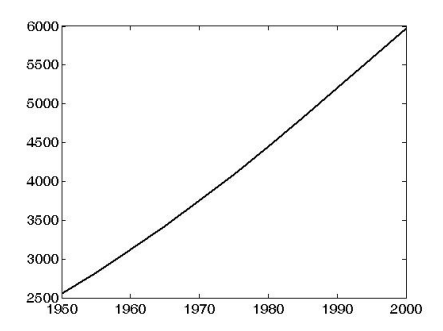
\includegraphics[width=0.5\linewidth]{fig_18_14}
		\label{fig:fig_18_14}
	\end{figure}
	\bigbreak



\section{}
	\bigbreak
A MATLAB M-file for the fourth-order RK method can be developed as
	\bigbreak
\begin{lstlisting}[numbers=none]
function [t,y] = rk4(dydt,tspan,y0,h)
%	 [t,y] = rk4(dydt,tspan,y0,h):
%		 uses the fourth-order Runge-Kutta method to integrate an ODE
% input:
%	 dydt = name of the M-file that evaluates the ODE
%	 tspan = [ti, tf] where ti and tf = initial and
%		 final values of independent variable
%	 y0 = initial value of dependent variable
%	 h = step size
% output:
%	 t = vector of independent variable
%	 y = vector of solution for dependent variable


ti = tspan(1);
tf = tspan(2);
t = (ti:h:tf)';
n = length(t);
% if necessary, add an additional value of t
% so that range goes from t = ti to tf
if t(n)<tf
	 t(n+1) = tf;
	 n = n+1;
end
y = y0*ones(n,1); %preallocate y to improve efficiency
for i = 1:n-1
	 hh = t(i+1) - t(i);
	 k1 = feval(dydt,t(i),y(i));
	 ymid = y(i) + k1*hh/2;
	 k2 = feval(dydt,t(i)+hh/2,ymid);
	 ymid = y(i) + k2*hh/2;
	 k3 = feval(dydt,t(i)+hh/2,ymid);
	 yend = y(i) + k3*hh;
	 k4 = feval(dydt,t(i)+hh,yend);
	 phi = (k1+2*(k2+k3)+k4)/6;
	 y(i+1) = y(i) + phi*hh;
end
plot(t,y) 
\end{lstlisting}
	\bigbreak
Here is the test of the solution of Prob \ref{sec:sec_18_2} First, an M-file holding the differential
equation is written as
	\bigbreak
\begin{lstlisting}[numbers=none]
function dy = dydx(x, y)
dy = (1+2*x)*sqrt(y);
\end{lstlisting}
	\bigbreak
Then the M-file can be invoked as in 
	\bigbreak
\begin{lstlisting}[numbers=none]
>> [x,y] = rk4(@dydx,[0 1],1,0.1);
>> disp([x,y])
	 0		 1.0000
	 0.1000 	1.1130
	 0.2000 	1.2544
	 0.3000 	1.4280
	 0.4000 	1.6384
	 0.5000 	1.8906
	 0.6000 	2.1904
	 0.7000 	2.5440
	 0.8000 	2.9584
	 0.9000 	3.4410
	 1.0000 	4.0000
\end{lstlisting}
	\bigbreak
The following plot is generated
	\bigbreak
	\begin{figure}[H]
		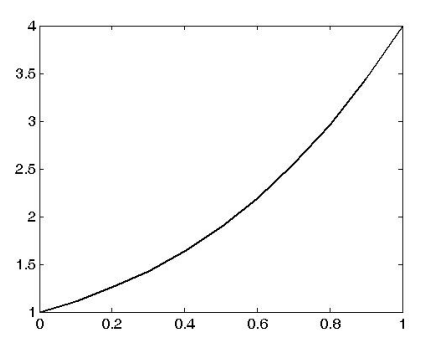
\includegraphics[width=0.5\linewidth]{fig_18_15}
		\label{fig:fig_18_15}
	\end{figure}
	\bigbreak



\section{}
\begin{blockquote}
 Note that students can take two approaches to developing this M-file. The first program
shown below is strictly developed to solve 2 equations. 
\end{blockquote}
	\bigbreak
\begin{lstlisting}[numbers=none]
function [t,y1,y2] = rk42(dy1dt,dy2dt,tspan,y10,y20,h)
% 	[t,y1,y2] = rk42(dy1dt,dy2dt,tspan,y10,y20,h):
% 		uses the fourth-order RK method to integrate a pair of ODEs
% input:
% 	dy1dt = name of the M-file that evaluates the first ODE
% 	dy2dt = name of the M-file that evaluates the second ODE
% 	tspan = [ti, tf] where ti and tf = initial and
% 		final values of independent variable
% 	y10 = initial value of first dependent variable
% 	y20 = initial value of second dependent variable
%	 h = step size
% output:
%	 t = vector of independent variable
%	 y1 = vector of solution for first dependent variable
%	 y2 = vector of solution for second dependent variable
ti = tspan(1);
tf = tspan(2);
t = (ti:h:tf)';
n = length(t);
% if necessary, add an additional value of t
% so that range goes from t = ti to tf
if t(n)<tf
	 t(n+1) = tf;
	 n = n+1;
end
y1 = y10*ones(n,1); %preallocate y's to improve efficiency
y2 = y20*ones(n,1);
for i = 1:n-1
	 hh = t(i+1) - t(i);
	 k11 = feval(dy1dt,t(i),y1(i),y2(i));
	 k12 = feval(dy2dt,t(i),y1(i),y2(i));
	 ymid1 = y1(i) + k11*hh/2;
	 ymid2 = y2(i) + k12*hh/2;
	 k21 = feval(dy1dt,t(i)+hh/2,ymid1,ymid2);
	 k22 = feval(dy2dt,t(i)+hh/2,ymid1,ymid2);
	 ymid1 = y1(i) + k21*hh/2;
	 ymid2 = y2(i) + k22*hh/2;
	 k31 = feval(dy1dt,t(i)+hh/2,ymid1,ymid2);
	 k32 = feval(dy2dt,t(i)+hh/2,ymid1,ymid2);
	 yend1 = y1(i) + k31*hh;
	 yend2 = y2(i) + k32*hh;
	 k41 = feval(dy1dt,t(i)+hh,yend1,yend2);
	 k42 = feval(dy2dt,t(i)+hh,yend1,yend2);
	 phi1 = (k11+2*(k21+k31)+k41)/6;
	 phi2 = (k12+2*(k22+k32)+k42)/6;
	 y1(i+1) = y1(i) + phi1*hh;
	 y2(i+1) = y2(i) + phi2*hh;
end
plot(t,y1,t,y2,'--')
\end{lstlisting}
	\bigbreak
Here is the test of the solution of Prob. \ref{sec:sec_18_7} First, M-files holding the differential equations
are written as
	\bigbreak
\begin{lstlisting}[numbers=none]
function dy = dy1dt(t, y1, y2)
dy = -2*y1 + 5*y2*exp(-t);


function dy = dy2dt(t, y1, y2)
dy = -y1*y2^2/2; 
\end{lstlisting}
	\bigbreak
Then the M-file can be invoked as in
	\bigbreak
\begin{lstlisting}[numbers=none]
>> [t,y1,y2]=rk42(@dy1dt,@dy2dt,[0 0.4],2,4,0.1);
>> disp([t,y1,y2])
 		0	 2.0000	 4.0000
	 0.1000	 3.0410	 2.6286
	 0.2000	 3.3426	 1.8453
	 0.3000	 3.3020	 1.4106
	 0.4000	 3.1078	 1.1500 
\end{lstlisting}
	\bigbreak
The following plot is generated 
	\bigbreak
	\begin{figure}[H]
		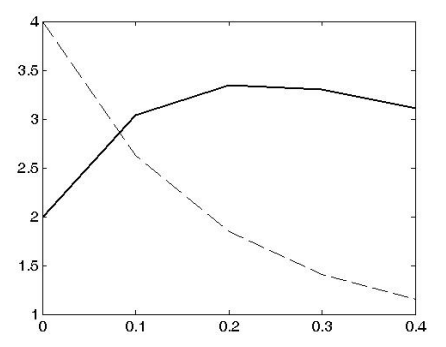
\includegraphics[width=0.5\linewidth]{fig_18_16}
		\label{fig:fig_18_16}
	\end{figure}
	\bigbreak
A better approach is to develop an M-file that can be used for any number of simultaneous
first-order ODEs as in the following code: 
	\bigbreak
\begin{lstlisting}[numbers=none]
function [t,y] = rk4sys(dydt,tspan,y0,h)
% 	[t,y] = rk4sys(dydt,tspan,y0,h):
%		 uses the fourth-order RK method to integrate a pair of ODEs
% input:
%	 dydt = name of the M-file that evaluates the ODEs
%	 tspan = [ti, tf] where ti and tf = initial and
%		 final values of independent variable
%	 y0 = initial values of dependent variables
%	 h = step size
% output:
%	 t = vector of independent variable
%	 y = vector of solution for dependent variables


ti = tspan(1);
tf = tspan(2);
t = (ti:h:tf)';
n = length(t);
% if necessary, add an additional value of t
% so that range goes from t = ti to tf
if t(n)<tf
	 t(n+1) = tf;
	  n = n+1;
end
y(1,:) = y0;
for i = 1:n-1
	 hh = t(i+1) - t(i);
	 k1 = feval(dydt,t(i),y(i,:))';
	 ymid = y(i,:) + k1*hh/2;
	 k2 = feval(dydt,t(i)+hh/2,ymid)';
	 ymid = y(i,:) + k2*hh/2;
	 k3 = feval(dydt,t(i)+hh/2,ymid)';
	 yend = y(i,:) + k3*hh;
	 k4 = feval(dydt,t(i)+hh,yend)';
	 phi = (k1+2*(k2+k3)+k4)/6;
	 y(i+1,:) = y(i,:) + phi*hh;
end
plot(t,y(:,1),t,y(:,2),'--')
\end{lstlisting}
	\bigbreak
This code solves as many ODEs as are specified. Here is the test of the solution of Prob. \ref{sec:sec_18_7}. First, a single M-file holding the differential equations can be written as 
	\bigbreak
\begin{lstlisting}[numbers=none]
function dy = dydtsys(t, y)
dy = [-2*y(1) + 5*y(2)*exp(-t);-y(1)*y(2)^2/2]; 
\end{lstlisting}
	\bigbreak
Then the M-file can be invoked as in
	\bigbreak
\begin{lstlisting}[numbers=none]
>> [t,y]=rk4sys(@dydtsys,[0 0.4],[2 4],0.1);
>> disp([t,y])
		0 	 2.0000 	 4.0000
	 0.1000	 3.0410	 2.6286
	 0.2000	 3.3426	 1.8453
	 0.3000	 3.3020	 1.4106
	 0.4000	 3.1078	 1.1500 
\end{lstlisting}
\end{document}